\chapter[Processo de Engenharia de Requisitos]{Processo de Engenharia de Requisitos}

O processo de Engenharia de Requisitos foi estabelecido com base no SAFe combinado com o \textit{Scrum}.

O SAFe é dividido em três níveis: Portfólio, Programa e Time. Em cada nível são representados os requisitos
em diferentes graus de abstração, como: Temas de Investimento, Épicos, \textit{Features} e Histórias.
Cada nível também possui papéis responsáveis por criar e manter esses requisitos, como: \textit{Product Portfolio Manager}, 
\textit{Product Manager} e \textit{Product Owner}. O SAFe é baseado no \textit{Scrum} e
possui características, alguns artefatos e papéis semelhantes. \cite{safe}

% A estrutura geral do SAFe pode ser vista na Figura \ref{fig:safe}
% 
% \begin{figure}[!htb]
% \centering
% 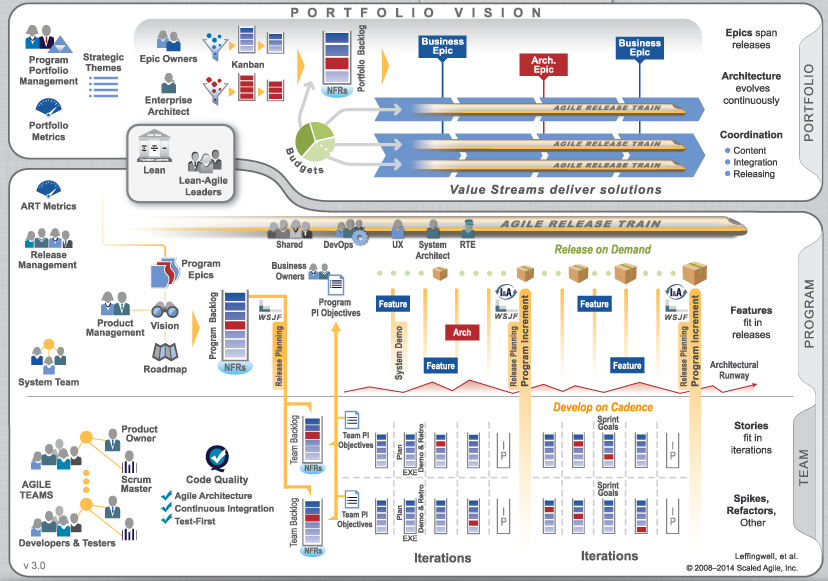
\includegraphics[scale=0.7]{figuras/safe.png}
% \caption{\textit{Big Picture} SAFe. Fonte: \cite{safe}}
% \label{fig:safe}
% \end{figure}

O \textit{Scrum} é formado por eventos, papéis e artefatos. Os eventos são: \textit{Sprint}, Reunião de Planejamento
da \textit{Sprint}, Reunião diária e Reunião de Retrospectiva da \textit{Sprint}. Os papéis são: \textit{Product Owner},
\textit{Scrum Master} e Time de Desenvolvimento. Os artefatos são: \textit{Backlog} do Produto, \textit{Backlog da Sprint} e Incremento. \cite{scrum}.
% Os eventos e artefatos do Scrum pode ser vista na Figura \ref{fig:scrum}
% 
% \begin{figure}[!htb]
% \centering
% 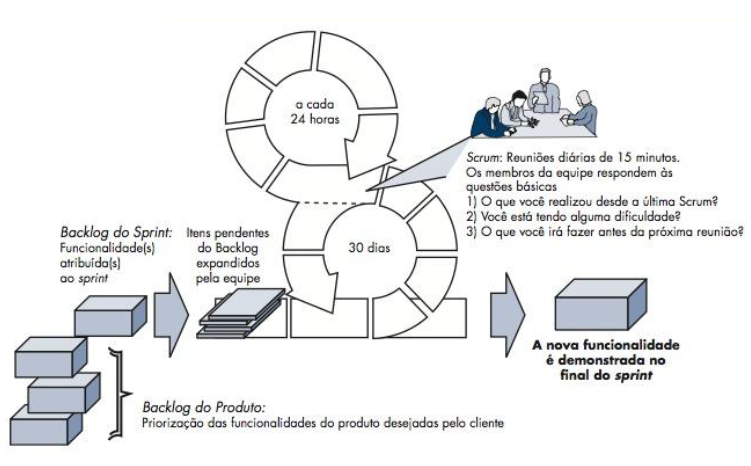
\includegraphics[scale=0.7]{figuras/scrum.png}
% \caption{Eventos e artefatos do Scrum. Fonte: \cite{pressman}}
% \label{fig:scrum}
% \end{figure}


Dessa forma, foi estabelecido um processo, que pode ser visto na Figura \ref{fig:Processo}, adequado ao contexto do trabalho.
É composto das seguintes atividades: Estabelecer Tema de Investimento, Levantar épicos, Levantar \textit{Features},
Construir Visão, Construir \textit{Roadmap}, Identificar Requisitos Não Funcionais,Escrever
Histórias e Planejar \textit{Release} e no subprocesso Executar Iteração tem Planejar Iteração,
Especificar Histórias, Desenvolver Histórias, Realizar Revisão da Iteraç\~ao e Realizar Retrospectiva da 
Iteração. Nas Figuras \ref{fig:Processo} e \ref{fig:iteracao} encontram-se a versão mais atual do processo e as mudanças realizadas podem ser vistas no Apêndice \ref{mudancas_processo}.

\pagebreak
\begin{figure}[!htb]
\flushleft
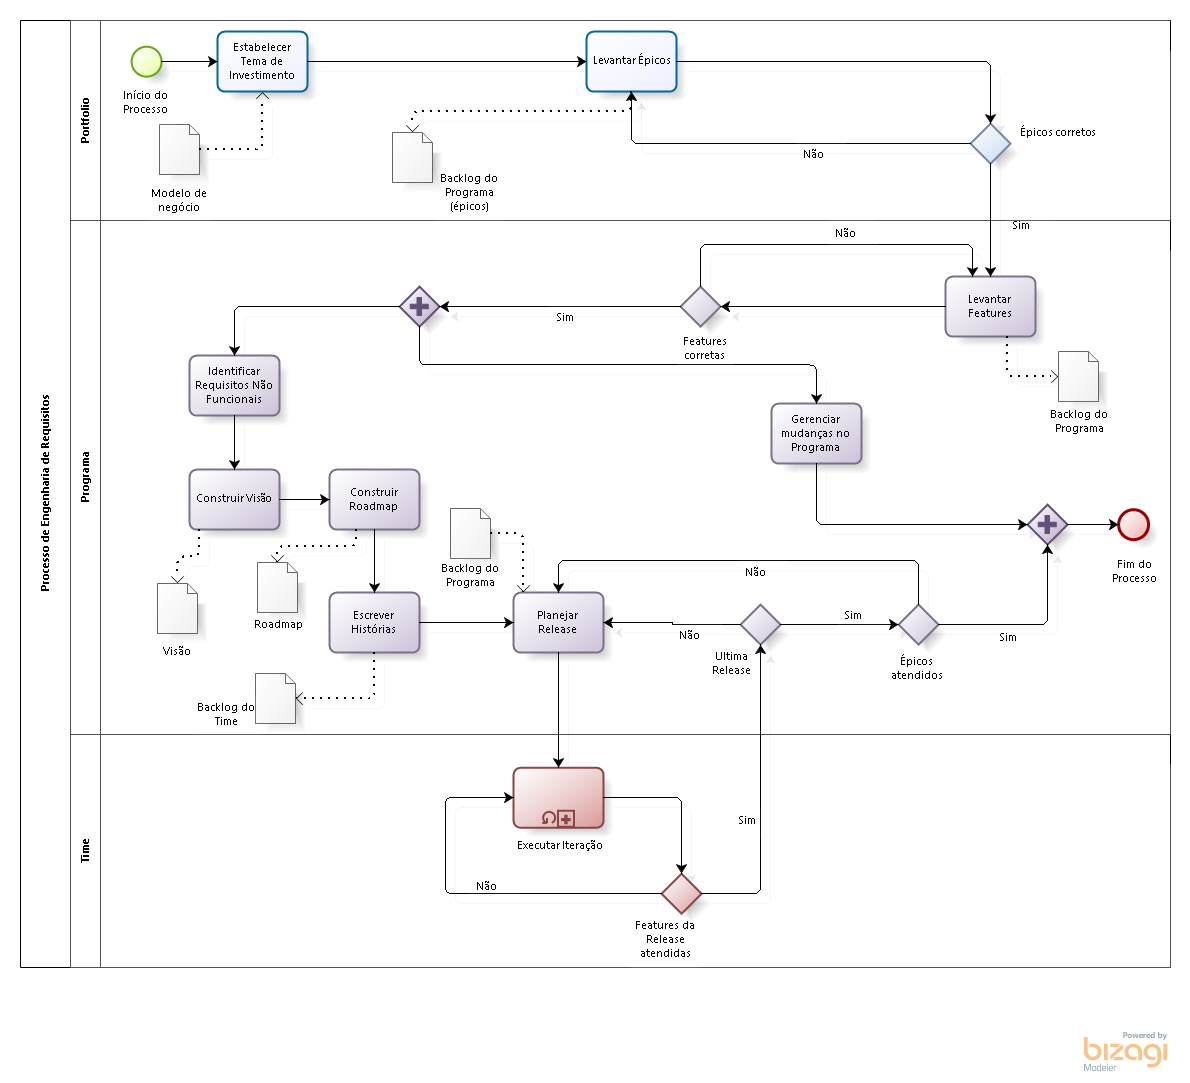
\includegraphics[scale=0.6]{figuras/processo3.png}
\caption{Processo de Engenharia de Requisitos - Versão 2.0}
\label{fig:Processo}
\end{figure}

\begin{figure}[!htb]
\flushleft
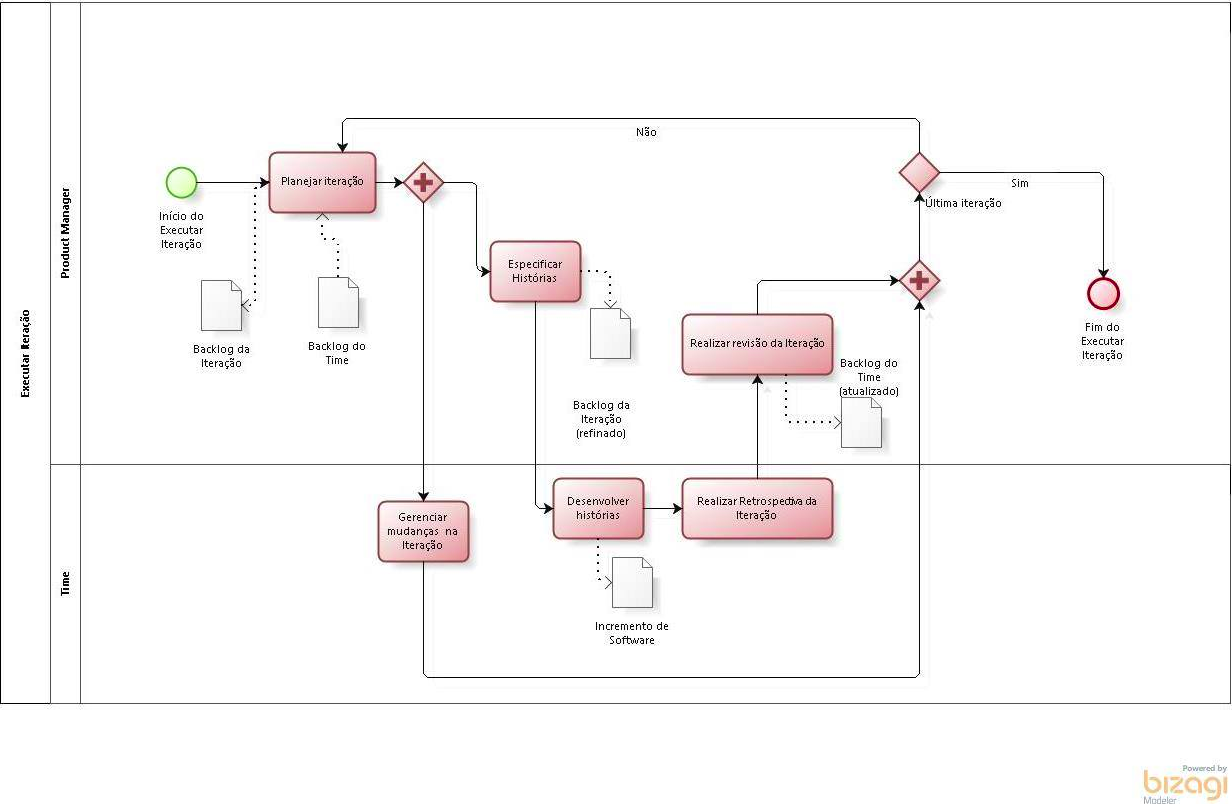
\includegraphics[scale=0.4]{figuras/iteracao2.png}
\caption{Suprocesso Executar Iteração - Versão 2.0}
\label{fig:iteracao}
\end{figure}

\pagebreak


% \section{Atividades}

\subsection{Estabelecer Tema de Investimento}

  \textbf{Descrição}: Essa atividade consiste na definição do tema de investimento a partir do \textit{Workshop} de Requisitos realizado.\\

  \textbf{Tarefas}:

  \begin{itemize}
  
    \item \indent \textit{Fazer Análise Documental}: Analisar documentos da empresa e o modelo de negócios produzido pela equipe de Modelagem.
   
   \item \indent \textit{Fazer Workshop de Requisitos}: Reunião com o cliente e o time para levantar requisitos de mais alto nível. Consiste
   em uma técnica de elicitação definida no Capítulo \ref{tecnicas}.

   \item \indent \textit{Validar Tema de Investimento}: Escrever o tema de investimento e confirmar com o cliente se
   o Tema de Investimento estabelecido está correto.
  \end{itemize}

  \textbf{Participantes}: \textit{Product Manager}, \textit{Scrum Master}, Time \\

  \textbf{Artefatos de Entrada}: Modelo de negócio \\

  \textbf{Artefatos de Saída}: Tema de Investimento\\

\subsection{Levantar Épicos}
  \textbf{Descrição}: Essa atividade consiste no levantamento dos épicos com o \textit{Product Manager} através do  \textit{Workshop} de Requisitos. \\

  \textbf{Tarefas}:

  \begin{itemize}
   \item \indent \textit{Fazer Workshop de Requisitos}: Reunião com o cliente e o time para levantar requisitos de mais alto nível. Consiste
   em uma técnica de elicitação definida no Capítulo \ref{tecnicas}.

   \item \indent \textit{Escrever Épicos}: A partir das anotações feitas no \textit{Workshop},
   escrever os épicos no \textit{Backlog} do Programa.
   
   \item \indent \textit{Manter Rastreabilidade}: Registrar na ferramenta cada épico como derivado do tema de investimento.

  \end{itemize}

  \textbf{Participantes}: \textit{Product Manager}, \textit{Scrum Master}, Time \\

  \textbf{Artefatos de Entrada}: Anotações do \textit{Workshop} \\

  \textbf{Artefatos de Saída}: \textit{Backlog} do Programa (Épicos) \\

\subsection{Fazer reunião de validação dos épicos}
  \textbf{Descrição}: Essa atividade consiste na apresentação dos épicos especificados para o \textit{Product Manager}, de modo a validar se os épicos
  especificados estão corretos e correspondem ao esperado. \\

  \textbf{Tarefas}:

  \begin{itemize}
    \item \indent \textit{Validar Épicos}: Confirmar em reunião com o cliente se os épicos estabelecidos estão corretos.

   \item \indent \textit{Escrever Épicos}: Se houver alguma mudança solicitada pelo cliente, escrever os épicos
   refinados no \textit{Backlog} do Programa.
  \end{itemize}

  \textbf{Participantes}: \textit{Product Manager}, \textit{Scrum Master}, Time \\

  \textbf{Artefatos de Entrada}: \textit{Backlog} do Programa (Épicos) \\

  \textbf{Artefatos de Saída}:  \textit{Backlog} do Programa (Épicos) \\

\subsection{Levantar \textit{Features}}
\textbf{Descrição}: Essa atividade consiste em listar as \textit{Features}, a partir dos épicos ,
que são as tarefas ou os “serviços” que o sistema deve fornecer para atender as necessidades das partes interessadas.
Deve-se observar se as \textit{features} condizem com ou traduzem de forma clara os Épicos
definidos previamente, e se através delas é possível escrever as Histórias de Usuário.\\

\textbf{Tarefas}:

  \begin{itemize}
   \item \indent \textit{Listagem de \textit{Features}}:  Listar \textit{Features} a partir dos Épicos de Portfólio ou a partir de outras \textit{Features}.

   \item \indent \textit{Adição e Edição de \textit{Features}}: Adicionar novas \textit{Features} ou modificar as \textit{Features} já levantas de acordo com as mudanças sugeridas na Reunião de Validação.

   \item \indent \textit{Manter Rastreabilidade}: Registrar na ferramenta de qual épico é cada \textit{Feature}.
   \end{itemize}

\textbf{Participantes}: \textit{Product Manager}, \textit{Scrum Master}, Time \\

\textbf{Artefatos de Entrada}: \textit{Backlog} do Programa (Épicos) \\

\textbf{Artefatos de Saída}:   \textit{Backlog} do Programa (\textit{Features}) \\

\subsection{Fazer reunião de validação das \textit{features}}
  \textbf{Descrição}: Essa atividade consiste na apresentação das \textit{features} especificadas para o \textit{Product Manager}, de modo a validar se
  estão corretos e correspondem ao esperado.  \\

  \textbf{Tarefas}:
  \begin{itemize}
   \item \indent \textit{Listagem de \textit{Features}}: Listar as \textit{Features} elicitadas e detalhadas até o momento;

   \item \indent \textit{Comparação \textit{Features}-Épicos}: Comparar as \textit{Features} e os Épicos, validando se as \textit{Features} expressam as iniciativas contidas nos Épicos;

   \item \indent \textit{Corrigir Possíveis Falhas}: Identificar equívocos no levantamento ou elicitação das \textit{Features} e propor mudanças.
  \end{itemize}

  \textbf{Participantes}: \textit{Product Manager}, \textit{Scrum Master}, Time \\

  \textbf{Artefatos de Entrada}: \textit{Backlog} do Programa (\textit{Features})\\

  \textbf{Artefatos de Saída}:   \textit{Backlog} do Programa (\textit{Features})\\

\subsection{Identificar Requisitos Não Funcionais}
  \textbf{Descrição}: Nesta atividade são identificados e descritos os requisitos não funcionais do sistema e são armazenados no \textit{Backlog} do Programa.  \\

  \textbf{Tarefas}:
  \begin{itemize}
   \item \indent \textit{Identificação de Requisitos não Funcionais}: Identificar e descrever os requisitos não funcionais

   \item \indent \textit{Armazenamento no \textit{Backlog}}: Armazenar no \textit{Backlog} do Programa
  \end{itemize}

  \textbf{Participantes}: \textit{Product Manager}, \textit{Scrum Master}, Time \\

  \textbf{Artefatos de Entrada}:  Não se aplica\\

  \textbf{Artefatos de Saída}:  \textit{Backlog} do Programa (Requisitos Não Funcionais)\\

\subsection{Construir Visão}
  \textbf{Descrição}: Nesta atividade, deve-se compilar as \textit{Features}, com os requisitos não funcionais, incluindo elementos
  regulatórios ou outros padrões de conformidade, e qualquer restrição de design. A partir disso, é possível descrever um panorama da solução a
  ser desenvolvida, refletindo as necessidades das partes interessadas e os recursos propostos para atender essas necessidades. \\

  \textbf{Tarefas}:
  \begin{itemize}
   \item \indent \textit{Reunir Artefatos}: Reunir \textit{Features}, Requisitos não Funcionais, restrições e padrões.

   \item \indent \textit{Sintetizar e Integrar}: Sintetizar todas as Artefatos de entrada, integrando-as em uma visão holística (global) e coesa do projeto.

   \item \indent \textit{Planejamento do \textit{RoadMap}}: Planejar o \textit{RoadMap} de entregas das \textit{Features}.
  \end{itemize}

  \textbf{Participantes}: \textit{Product Manager}, \textit{Scrum Master}, Time \\

  \textbf{Artefatos de Entrada}: \textit{Backlog} do Programa \\

  \textbf{Artefatos de Saída}:  Documento de Visão\\

\subsection{Construir \textit{Roadmap}}
  \textbf{Descrição}: A partir da Visão, deve-se elaborar uma espécie de roteiro, que situa e comunica a equipe e o programa em relação ao
  alinhamento dos objetivos de negócios, e fornece visibilidade das entregas ao longo de um cronograma de curto prazo.
  Esse roteiro divide as \textit{features} nas \textit{Releases}. \\

  \textbf{Tarefas}:
  \begin{itemize}
   \item \indent \textit{Reunir Documento de Visão}: Reunir o documento de visão

   \item \indent \textit{Definir Prioridades}: Priorizar \textit{Features} no \textit{Backlog} do programa.

   \item \indent \textit{Alocamento de \textit{Features}}: Alocar \textit{Features} em \textit{Releases}.

   \item \indent \textit{Escrever}: Escrever histórias
  \end{itemize}

  \textbf{Participantes}: \textit{Product Manager}, \textit{Scrum Master}, Time \\

  \textbf{Artefatos de Entrada}: Documento de Visão \\

  \textbf{Artefatos de Saída}:  \textit{Roadmap}\\

\begin{figure}[!htb]
\centering
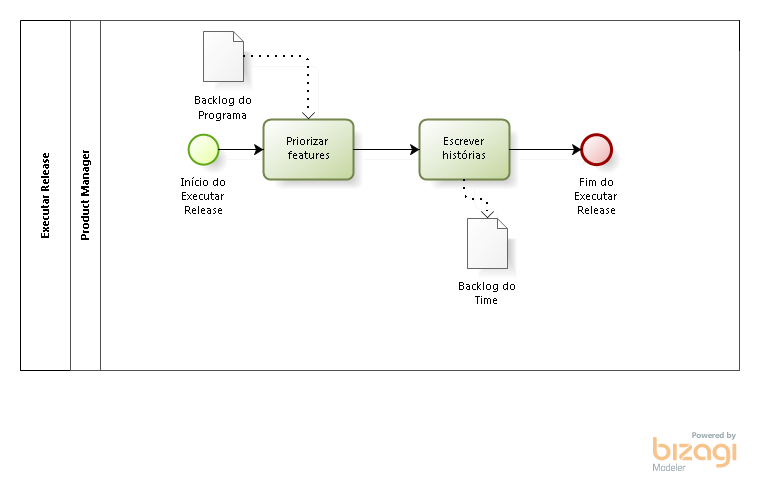
\includegraphics[scale=0.7]{figuras/release.png}
\caption{Subprocesso Executar \textit{Release}}
\label{fig:release}
\end{figure}

A partir do Subprocesso da Figura \ref{fig:release} o processo contém as seguintes atividades.

\subsection{Priorizar \textit{features}}
  \textbf{Descrição}: Essa atividade consiste na priorização das \textit{features} para a \textit{Release}. \\

  \textbf{Tarefas}:
  \begin{itemize}
   \item \indent \textit{Reunir \textit{Features}}: Reunir \textit{features} envolvidas na \textit{Release};

   \item \indent \textit{Estudar as \textit{Features}}: Estudar as \textit{features} para melhor entendimento de cada uma;

   \item \indent \textit{Definir Indicador de Complexidade}: Definir um identificador para saber quais demandam mais trabalho (horas de serviço);

   \item \indent \textit{Ordenar}: A partir dos resultados obtidos via análise, ordenar das que mostraram maiores métricas de esforço, até as menores, de modo que as mais difíceis sejam executadas o quanto antes.
  \end{itemize}

  \textbf{Participantes}: \textit{Product Manager}, \textit{Scrum Master}, Time\\

  \textbf{Artefatos de Entrada}: \textit{Backlog} do Programa \\

  \textbf{Artefatos de Saída}:  \textit{Backlog} do Programa \\

\subsection{Escrever histórias}
  \textbf{Descrição}: Essa atividade consiste na escrita das histórias em um nível macro, derivadas das \textit{features}, para composição do \textit{Backlog} do Time. \\

  \textbf{Tarefas}:
  \begin{itemize}
   \item \indent \textit{Identificar}: Identificar \textit{features};

   \item \indent \textit{Analisar}: Analisar o nível de prioridade das \textit{features};

   \item \indent \textit{Alocar}: Alocar \textit{features} nas iteração;

   \item \indent \textit{Instruir}: Auxílio do Scrum Master ao Product Manager a fim de ensinamento; de técnicas de escritas de histórias de usuário;

   \item \indent \textit{Escrita}: Escrever histórias;

   \item \indent \textit{Armazenamento}: Armazenar histórias no \textit{Backlog} do time.
   
   \item \indent \textit{Manter Rastreabilidade}: Registrar na ferramenta de qual \textit{Feature} é cada história.

  \end{itemize}

  \textbf{Participantes}: \textit{Product Manager}, \textit{Scrum Master}, Time\\

  \textbf{Artefatos de Entrada}: \textit{Backlog} do Programa \\

  \textbf{Artefatos de Saída}:   \textit{Backlog} do Time \\

\begin{figure}[!htb]
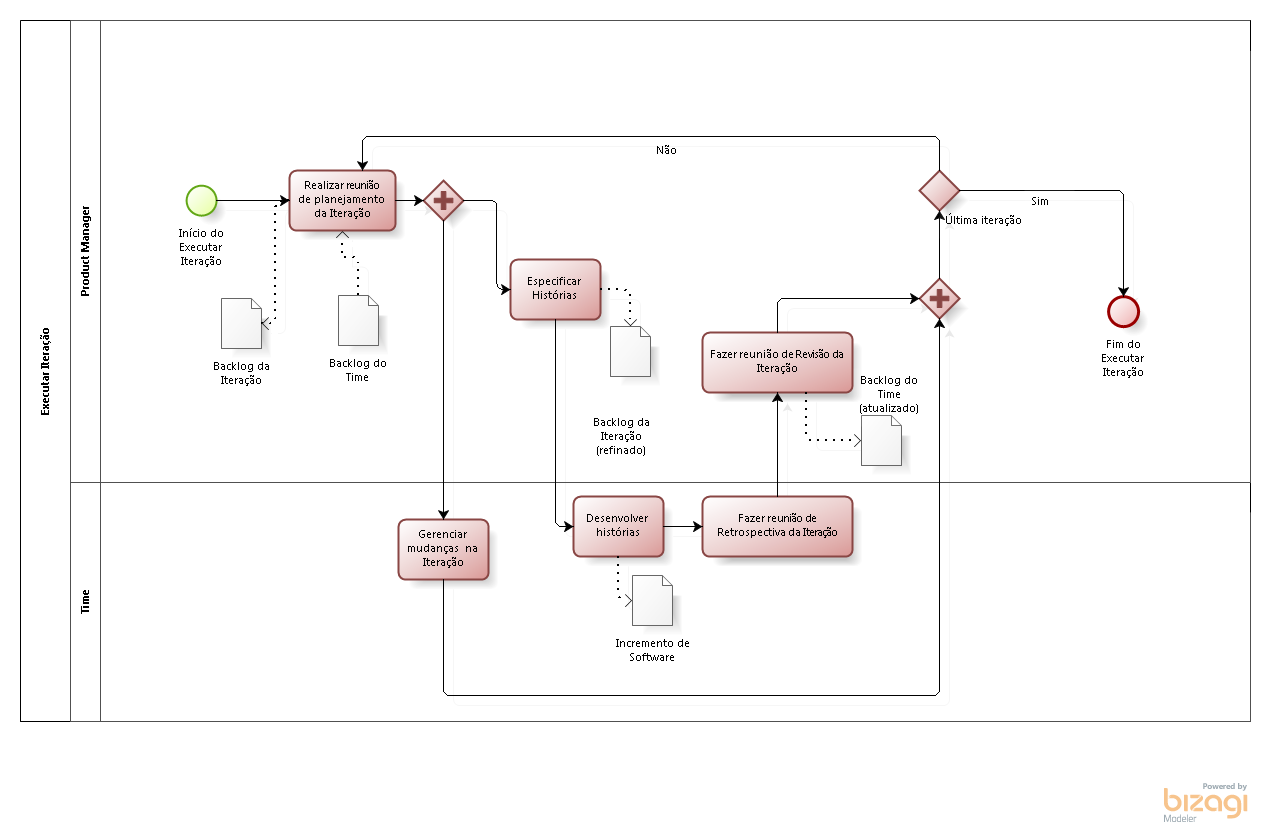
\includegraphics[scale=0.5]{figuras/iteracao.png}
\caption{Suprocesso Executar Iteração}
\label{fig:iteracao}
\end{figure}

A partir do Subprocesso da Figura \ref{fig:iteracao} o processo contém as seguintes atividades.

\subsection{Realizar reunião de planejamento da Iteração}
  \textbf{Descrição}: Essa atividade consiste no planejamento da iteração através da alocação das histórias definidas no \textit{Backlog} do Time para o \textit{Backlog} da iteração. \\

  \textbf{Tarefas}:
  \begin{itemize}
   \item \indent \textit{Alocação das Histórias}: Alocação das histórias no \textit{Backlog} da iteração

   \item \indent \textit{Armazenamento de Artefatos}: Armazenar no \textit{Backlog} de Iteração
  \end{itemize}

  \textbf{Participantes}: \textit{Product Manager}, \textit{Scrum Master}, Time\\

  \textbf{Artefatos de Entrada}: \textit{Backlog} do Time \\

  \textbf{Artefatos de Saída}:  \textit{Backlog} da Iteração\\

\subsection{Especificar histórias}
  \textbf{Descrição}: Essa atividade consiste na escrita mais detalhada das histórias que irão compor a
iteração. \\

  \textbf{Tarefas}:
  \begin{itemize}
   \item \indent \textit{Detalhamento das Histórias}: Detalhar histórias da iteração
   
   \item \indent \textit{Testes de aceitação}: Escrever testes de aceitação das histórias da iteração

   \item \indent \textit{Armazenamento de Artefatos}: Armazenar no \textit{Backlog} de Iteração

   \item \indent \textit{Atualizar}: Atualizar \textit{Backlog} do Time
  \end{itemize}

  \textbf{Participantes}: \textit{Product Manager}, \textit{Scrum Master}, Time\\

  \textbf{Artefatos de Entrada}: \textit{Backlog} da Iteração \\

  \textbf{Artefatos de Saída}:   \textit{Backlog} da Iteração\\

\subsection{Desenvolver histórias}
  \textbf{Descrição}: Essa atividade consiste no desenvolvimento e teste das histórias contidas no \textit{Backlog} da Iteração. Tem uma duração de 1 semana. \\

  \textbf{Tarefas}:

  \begin{itemize}
    \item \indent \textit{Desenvolver Histórias}: Implementar as histórias contidas no \textit{Backlog} da Iteração.

   \item \indent \textit{Testar Histórias}: Realizar testes unitários do código implementado na iteração e testes funcionais
   com base nos testes de aceitação.
  \end{itemize}

  \textbf{Participantes}: Time\\

  \textbf{Artefatos de Entrada}: \textit{Backlog} da Iteração \\

  \textbf{Artefatos de Saída}:   Incremento de Software\\

\subsection{Fazer reunião de revisão e retrospectiva da Iteração}
  \textbf{Descrição}: Essa atividade consiste na validação das histórias implementadas através da execução dos testes de aceitação. \\

  \textbf{Tarefas}:
  \begin{itemize}
   \item \indent \textit{Análise de Artefatos}: Analisar artefatos gerados na iteração;

   \item \indent \textit{Avaliar Pontos Positivos}: Definir pontos que ocorreram bem;

   \item \indent \textit{Definir Pontos de Melhoria}: Definir pontos que necessitam de melhoria;

   \item \indent \textit{Definir Novas Metas}: Definir novas metas de melhoria a serem alcançadas na nova iteração.
   
   \item \indent \textit{Atualizar o \textit{Backlog}}: Atualizar o \textit{Backlog} do Time.
  \end{itemize}

  \textbf{Participantes}: \textit{Product Manager}, Time\\

  \textbf{Artefatos de Entrada}: Incremento de Software \\

  \textbf{Artefatos de Saída}:   \textit{Backlog} do Time \\

% \section{Artefatos}

Os artefatos foram definidos de acordo com a proposta do SAFe feita por \citeonline{safe} e do Scrum feita 
por \citeonline{scrum}.

\begin{itemize}
  \item \textit{Backlog} do Programa
    \subitem O \textit{Backlog} do Programa é responsável por manter os épicos, as \textit{features} e os requisitos
    não funcionais. De acordo com \citeonline{safe}, o \textit{Backlog} do Programa mantém apenas as \textit{features} e os requisitos não funcionais,
    todavia para o processo definido a constituição deste \textit{Backlog} foi adaptado e ele passou a manter também
    os épicos. Essa escolha foi realizada para diminuir a quantidade de artefatos gerados. 
    
    Esse artefato é criado na atividade Levantar Épicos e 
    pode ser atualizado nas atividades: Fazer reunião de validação dos épicos, Levantar \textit{Features}, Especificar \textit{Features}, 
Fazer reunião de validação das \textit{Features}, Construir Visão, Construir \textit{Roadmap}, Identificar Requisitos Não Funcionais e durante as atividades
do subprocesso Executar \textit{Release}.
  
  \item Visão
   \subitem O Visão consiste em um documento que contém os requisitos funcionais, requisitos não funcionais, incluindo elementos regulatórios 
   ou outros padrões de conformidade, e qualquer restrição de design. Também contém um panorama da solução a ser desenvolvida, 
   refletindo as necessidades das partes interessadas e os recursos propostos para atender essas necessidades. \cite{safe}.
   No processo definido nesse trabalho é gerado na atividade Construir Visão.
  
  \item \textit{Roadmap}
     \subitem O \textit{Roadmap} consiste na alocação das \textit{features} em \textit{Releases}, através da determinação de datas e priorizações. \cite{safe}.
     O \textit{Roadmap} é definido na atividade: Construir \textit{Roadmap}.

    
  \item \textit{Backlog} do Time
      \subitem O \textit{Backlog} do Time é responsável por manter as histórias levantadas a partir das \textit{features}.  \cite{safe}. No processo definido
      é criado na atividade Escrever histórias na primeira \textit{Release} e pode ser atualizado nas atividades: Escrever histórias, Especificar histórias, Realizar reunião de planejamento 
      da Iteração, Fazer reunião de revisão e retrospectiva da Iteração.
  
  \item \textit{Backlog} da Iteração
        \subitem O \textit{Backlog} da Iteração é responsável por manter as histórias da iteração atual. \cite{safe}.
        No processo definido é criado na atividade Realizar reunião de planejamento 
      da Iteração e pode ser atualizado na atividade de Especificar histórias.
  
  \item Incremento de Software
      \subitem O Incremento de Software consiste na solução gerada a cada Iteração. \cite{scrum}. No processo definido é gerada na atividade de Desenvolver Histórias e validada na 
      atividade de Reunião de Revisão e retrospectiva da Iteração.
\end{itemize}

% \section{Papéis}

\begin{itemize}
  \item \textit{Product Manager} (PM)
 \subitem O \textit{Product Manager} consiste na equipe de Modelagem de Processos e foi escolhido
 para assumir também as responsabilidades do \textit{Product Owner} (PO). Essa escolha foi realizada
 levando em consideração que o PM está em um nível acima do PO. Com base no SAFe \cite{safe}, para
 esse processo suas responsabilidades são: \\
  \begin{enumerate}
    \item Definir o Tema de investimento;
    \item Levantar os Épicos;
    \item Levantar as \textit{Features};
    \item Definir o visão; 
    \item Criar o \textit{Roadmap}.
    \item Gerenciar a \textit{Release}; 
    \item Escrever as histórias;
    \item Validar os incrementos de software;
  \end{enumerate}
      
  \item \textit{Scrum Master}
 \subitem O  \textit{Scrum Master} é um membro da equipe de Requisitos. Esse papel foi escolhido
 para auxiliar o PM em suas atividades considerando que a equipe alocada para o papel não possui
 conhecimento sobre Requisitos. Assim, com base no Guia Scrum \cite{scrum}, para
 esse processo esse papel é responsável por: \\
    \begin{enumerate}
     \item Verificar se o processo está sendo realizado conforme planejado;
     \item Auxiliar o PM nas suas atividades; 
     \item Servir de elo de ligação entre o PM e o Time. 
    \end{enumerate}

  \item Time
 \subitem O  Time consiste na equipe de Requisitos e com base nas definições de \citeonline{safe}
 para esse processo, o time é responsável por: \\
    \begin{enumerate}
      \item Acompanhar as atividades de engenharia de Requisitos;
      \item Escrever os testes de aceitação das histórias;
      \item Desenvolver as histórias. 
    \end{enumerate}
      
\end{itemize}
